\section{Pilhas}

\begin{frame}
	\begin{block}{Pilhas}
		\begin{itemize}
			\item São estruturas de dados dinâmicas, como as listas ligadas, só que são mais simples e com algumas restrições adicionais.
			
			\item Seguem a lógica first in last out, uma analogia simples para entender as pilhas e suas restrições é imaginar uma pilha de pratos para serem limpos em um restaurante.
			
			\item O primeiro prato da pilha será o último a ser limpo, o último prato adicionado na pilha será o primeiro a ser limpo. Não deveria ser possível remover elementos intermediários de uma fila.... (para essa situação existem os deques.)
			
			\item Podem ser usadas em editores de texto com função “voltar”. Em games pode ser usada para salvar o jogo, guardando o estado do mundo em uma pilha permite retornar para ele de forma prática.
		\end{itemize}
	\end{block}
\end{frame}

\begin{frame}
	\begin{block}{Pilhas}
		\begin{figure}[!htb]
			\centering	  				
			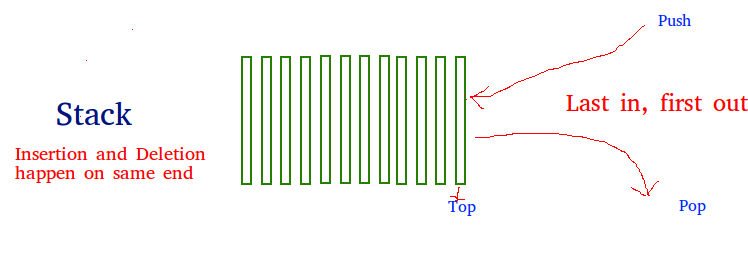
\includegraphics[height=3cm, width = 9cm]{./pic/stack.png}
			\caption{Exemplo de pilha \cite{GEEKS_2018}}
			\label{fig_pilha}
		\end{figure}
	\end{block}
\end{frame}

\begin{frame}
	\begin{block}{Pilhas}
		\begin{itemize}
			\item Programar em C\# com os alunos
			\item Mostrar complexidade no quadro
		\end{itemize}
	\end{block}
\end{frame}

\section{Filas}

\begin{frame}
	\begin{block}{Filas}
		\begin{itemize}
			\item São estruturas de dados dinâmicas, como as listas ligadas, só que são mais simples e com algumas restrições adicionais.
			
			\item Seguem a lógica: “Primeiro a entrar é o primeiro a sair”, uma analogia simples para entender as filas é uma fila de banco sem regras de cliente especial. Para contemplar os clientes especiais devemos considerar o uso de um deque.
			
			\item O primeiro cliente que chega será o primeiro cliente que será atendido, e assim por diante até acabar a fila.
			
			\item Processos sequenciais onde a ordem de chegada é relevante usam filas. 
		\end{itemize}
	\end{block}
\end{frame}


\begin{frame}
	\begin{block}{FIlas}
		\begin{figure}[!htb]
			\centering	  				
			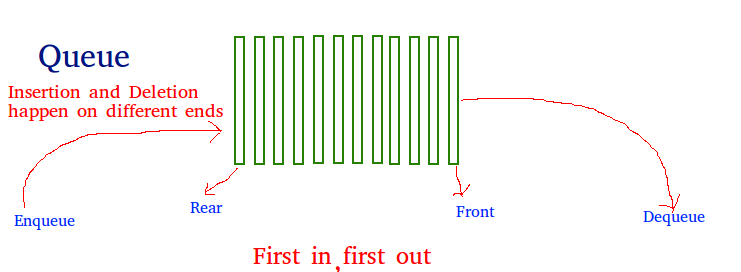
\includegraphics[height=3cm, width = 9cm]{./pic/queue.png}
			\caption{Exemplo de fila \cite{GEEKS_2018}}
			\label{fig_LLS_one}
		\end{figure}
	\end{block}
\end{frame}

\begin{frame}
	\begin{block}{Filas}
		\begin{itemize}
			\item Programar em C\# com os alunos
			\item Mostrar complexidade no quadro
		\end{itemize}
	\end{block}
\end{frame}